\documentclass[tikz,border=2pt]{standalone}
\usepackage{amsmath,amssymb}
\usepackage{tikz}
\usetikzlibrary{arrows.meta}

\begin{document}
% A vector space is closed under addition and scaling: from x and y one never leaves the
% space with x + y, cx, -x, 0. Many different objects obey the same axioms.
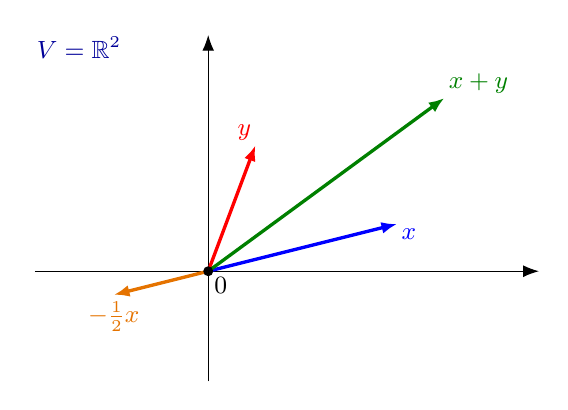
\begin{tikzpicture}[every node/.style={font=\small}, >={Latex[length=2mm]}]
	\node[blue!60!black, anchor=north west] at (-2.3,3.1) {$V=\mathbb{R}^2$};
	\draw[->] (-2.2,0) -- (4.2,0);
	\draw[->] (0,-1.4) -- (0,3.0);
	\draw[->, blue, very thick] (0,0) -- (2.4,0.6) node[below right, inner sep=1pt] {$x$};
	\draw[->, red, very thick] (0,0) -- (0.6,1.6) node[above left, inner sep=1pt] {$y$};
	\draw[->, green!50!black, very thick] (0,0) -- (3.0,2.2) node[above right, inner sep=1pt] {$x+y$};
	\draw[->, orange!90!black, very thick] (0,0) -- (-1.2,-0.3) node[below, inner sep=2pt] {$-\tfrac12x$};
	\fill (0,0) circle (1.8pt) node[below right, inner sep=2pt] {$0$};
\end{tikzpicture}
\end{document}
